\subsection{自更新盲密钥管理}
\label{subsec:sgxdedup-key-management}

每个客户端都通过一个共享的 \textit{ blinded} 密钥与密钥安全区安全通信,以防止密钥管理器 (\S\ref{subsec:sgxdedup-arch}) 窃听。 为了形成盲密钥,一种直接的方法是直接在密钥安全区和每个客户端之间实现密钥协商协议。 但是,密钥安全区需要即时验证客户端(例如,客户端可以更新或撤销其云服务订阅)。 这种动态认证给密钥安全区带来了性能负担。


\begin{figure}[t]
\centering
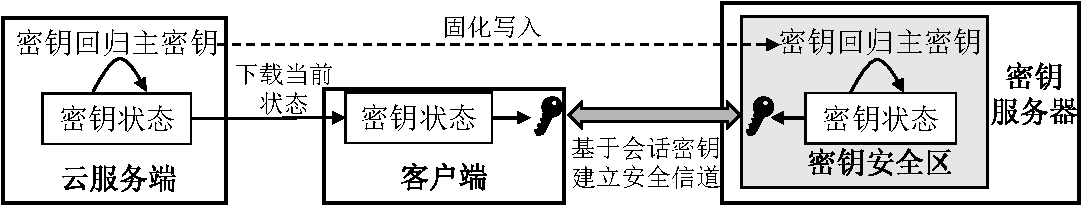
\includegraphics[width=\textwidth]{pic/sgxdedup/keyRegression.pdf}
\vspace{-16pt}
\caption{可更新的盲密钥管理概述:云端和密钥安全区可以根据其盲密钥导出新的盲密钥,而客户端只能从云端下载一个密钥状态,并访问最新的盲密钥。}
\label{fig:sgxdedup-keymanage}
\end{figure}

\sysnameS 在云的帮助下管理盲密钥。在初始化期间,云将一个不知情的秘密 $\kappa$ 硬编码到密钥安全区代码中。每个客户端从云端下载一个 \textit{ key state}(源自 $\kappa$;见下文),并生成其盲密钥(基于密钥状态)用于与密钥安全区的安全通信。本文的理由是双重的。首先,当客户端从云端发出任何下载请求时,云端可以检查客户端是否被授权。其次,本文可以从$\kappa$(而不是直接使用$\kappa$)派生一系列可更新的盲密钥,以防止被撤销/受损的客户端持续访问密钥安全区。作为附带的好处,可更新密钥管理还可以防止在线暴力攻击 (\S\ref{subsec:sgxdedup-encrypted-dedup}),而不会主动降低密钥生成速率 \cite{bellare2013DupLESS}。

\sysnameS 使用 \textit{ key regression} \cite{fu06} 导出可更新的盲密钥,同时确保每个客户端和密钥安全区中的盲密钥是一致的。具体来说,密钥回归适用于一系列密钥状态 $S[1]、S[2]、\ldots、S[m]$,每个状态都可用于派生密钥(例如,通过散列)。它允许密钥安全区和云执行 \textit{ rekeying} 以使用 \textit{ 密钥回归秘密从旧状态导出新状态(例如,从 $S[1]$ 导出 $S[2]$) },这样客户端就无法在不知道关键回归秘密的情况下了解有关新状态的任何信息。它还允许每个客户端从新状态派生任何旧状态(例如,从 $S[2]$ 派生 $S[1]$)。

为了在 \sysnameS 中实现密钥回归,本文使用 $\kappa$ 作为在云和密钥安全区之间共享的密钥回归秘密,用于派生新的状态和密钥。在每次上传时,客户端首先从云端下载最新的密钥状态$S[i]$,并请求密钥安全区接受的盲密钥的当前版本号$j$。鉴于密钥安全区可能无法及时更新盲密钥(例如,它正忙于在计划的更新密钥时间内准确地为密钥生成提供服务),$j$ 通常小于 $i$(即 $S[j]$在 $S[i]$) 之前。然后客户端从$S[i]$和对应的盲密钥$K[j]$推导出$S[j]$,并基于相同的$K[j]$与密钥安全区通信。请注意,云可以派生$K[j]$,但它不能窃听每个客户端和密钥安全区之间的通信,因为通过客户端和密钥管理器之间的基于 SSL/TLS 的通道额外保护了通信(参见本文在 \S\ref{subsec:sgxdedup-threat} 中的假设)。

\sysnameS 更新云和密钥安全区中的盲密钥。 云实现了一个计时器,以在周期性的时间间隔内触发密钥更新。 密钥管理器发出 \textit{ rekeying ECall} 以在达到预定的密钥更新时间时触发密钥更新。

目前,本文实现了基于哈希的密钥回归方案 \cite{fu06} 以获得高密钥派生性能。 具体来说,本文定义了一个参数 $n$(现在设置为 $2^{20}$ \cite{fu06})来指示可承受的最大密钥更新次数。 云和密钥安全区计算第 i 个密钥状态为 $S[i] = {\bf H}^{n-i+1}(\kappa)$,每个客户端派生相应的盲密钥为 $K[i] = {\bf H}(S[i] || 0^8)$,其中${\bf H}^{n-i+1}()$迭代调用密码散列函数${ \bf H}()$ 乘以 $n-i+1$ 次,$||$ 是连接运算符。 为了导出旧状态,客户端下载 $S[i]$ 并恢复 $S[i-1] = {\bf H}(S[i])$。
